%Victor Vermès
On dit que deux carrés \emph{se touchent} s'ils ont au moins un point de leurs bords respectifs en commun. Autour d'un carré de côté $1$, il est possible de placer $8$ autres carrés de côté $1$ touchant le premier, sans jamais que deux carrés ne se superposent. Il suffit de placer les carrés comme dans un échiquier.

Est-il possible d'en placer $9$ ?

\begin{figure}[h!]
\centering
\tikzstyle{my help lines}=[gray,thick,dashed]
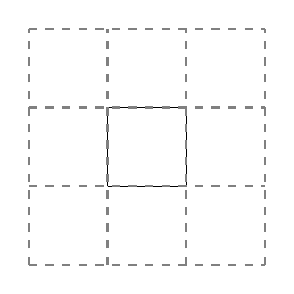
\begin{tikzpicture}[scale=1]
\draw (0,0) grid (1,1);
\draw[style=my help lines] (-1,-1) grid (2,2);
\end{tikzpicture}
\caption{Exemple : $8$ carrés qui \emph{touchent} le carré central sans se superposer}
\end{figure}